\documentclass[handout,aspectratio=169]{beamer}
\usepackage[english]{babel}
\usepackage{metalogo}
\usepackage{listings}
\usepackage{fontspec}
\usepackage{tikz}
\usepackage{graphicx}
\usepackage{subcaption}
%%%%%%%%%%%%%%%%%%%%%%%%%%%%%%%%%%%%%%%%%%%%%%%%%%%%%%%%%%%%%%%%%%%%%%%%%%%%%%%%%%%%%%%%
%%%%%%%%%%%%%%%%%%%%%%%%%%%%%%%%%%%%%%%%%%%%%%%%%%%%%%%%%%%%%%%%%%%%%%%%%%%%%%%%%%%%%%%%
%%%%%%%%%%%%%%%%%%%%%%%%%%%%%%%%%%%%%%%%%%%%%%%%%%%%%%%%%%%%%%%%%%%%%%%%%%%%%%%%%%%%%%%%
\usepackage{xcolor}
\definecolor{BK}{HTML}{3b3838}
\definecolor{Blue}{RGB}{88, 105, 225}
\newcommand{\BK}[1]{\color{BK} #1}
\newcommand{\URed}[1]{\color{URed} #1}
\newcommand{\white}[1]{\color{white} #1}
\newcommand{\Orange}[1]{\color{QOrange} #1}
\newcommand{\blue}[1]{\color{blue} #1}
\newcommand{\Blue}[1]{\color{Blue} #1}
\newcommand{\red}[1]{\color{red} #1}
\newcommand{\gray}[1]{\color{gray} #1}
\newcommand{\orange}[1]{\color{orange} #1}
\usepackage{accents}
\newcommand\thickbar[1]{\accentset{\rule{.4em}{.8pt}}{#1}}
\newcommand{\ubar}[1]{\underaccent{\bar}{#1}}
\newcommand{\hatbar}[1]{\bar{\hat{#1}}}
\newcommand{\hatubar}[1]{\underaccent{\bar}{\hat{#1}}}
\newcommand{\ul}[1]{\underline{#1}}
\newcommand{\ol}[1]{\overline{#1}}
%%%%%%%%%%%%%%%%%%%%%%%%%%%%%%%%%%%%%%%%%%%%%%%%%%%%%%%%%%%%%%%%%%%%%%%%%%%%%%%%%%%%%%%%
\newcommand{\bO}[1]{\bf \Orange #1}
%%%%%%%%%%%%%%%%%%%%%%%%%%%%%%%%%%%%%%%%%%%%%%%%%%%%%%%%%%%%%%%%%%%%%%%%%%%%%%%%%%%%%%%%
%%%%%%%%%%%%%%%%%%%%%%%%%%%%%%%%%%%%%%%%%%%%%%%%%%%%%%%%%%%%%%%%%%%%%%%%%%%%%%%%%%%%%%%%
\newcommand{\YBox}[3]{
\begin{center}
\begin{minipage}{#1\linewidth}
\begin{exampleblock}{#2}
    #3
\end{exampleblock}
\end{minipage}
\end{center}
}

\newcommand{\OBox}[3]{
\begin{center}
\begin{minipage}{#1\linewidth}
\begin{block}{#2}
    #3
\end{block}
\end{minipage}
\end{center}
}

\newcommand{\Columns}[4]{
\begin{columns}
\begin{column}{#1\textwidth}
#2
\end{column}
\begin{column}{#3\textwidth}  %%<--- here
#4
\end{column}
\end{columns}
}
%%%%% NEW MATH DEFINITIONS %%%%%

\usepackage{amsmath,amsfonts,bm}
\usepackage{amssymb}

%%%%%%%%%%%%%%%%%%%%%%%%%%%%%%%%%%%%%%%%%%%%%%%%%%%%%%%%%%%%%%%%%%%%%%%%%%%%%%%%
%%%%%%%%%%%%%%%%%%%%%%%%%%%%%%%%%%%%%%%%%%%%%%%%%%%%%%%%%%%%%%%%%%%%%%%%%%%%%%%%
\usepackage{natbib}
\usepackage{ulem}
% \usepackage{cite}
\usepackage{amsmath,amssymb,amsfonts}
\usepackage{algorithm,algorithmicx,algpseudocode}
\usepackage{graphicx}
% \usepackage{subcaption}
\usepackage{mwe}
\usepackage{textcomp}
\usepackage{xcolor}
\usepackage{dsfont}
\usepackage{bbm}
% Mark sections of captions for referring to divisions of figures
\newcommand{\figleft}{{\em (Left)}}
\newcommand{\figcenter}{{\em (Center)}}
\newcommand{\figright}{{\em (Right)}}
\newcommand{\figtop}{{\em (Top)}}
\newcommand{\figbottom}{{\em (Bottom)}}
\newcommand{\captiona}{{\em (a)}}
\newcommand{\captionb}{{\em (b)}}
\newcommand{\captionc}{{\em (c)}}
\newcommand{\captiond}{{\em (d)}}

% Highlight a newly defined term
\newcommand{\newterm}[1]{{\bf #1}}


% Figure reference, lower-case.
\def\figref#1{figure~\ref{#1}}
% Figure reference, capital. For start of sentence
\def\Figref#1{Figure~\ref{#1}}
\def\twofigref#1#2{figures \ref{#1} and \ref{#2}}
\def\quadfigref#1#2#3#4{figures \ref{#1}, \ref{#2}, \ref{#3} and \ref{#4}}
% Section reference, lower-case.
\def\secref#1{section~\ref{#1}}
% Section reference, capital.
\def\Secref#1{Section~\ref{#1}}
% Reference to two sections.
\def\twosecrefs#1#2{sections \ref{#1} and \ref{#2}}
% Reference to three sections.
\def\secrefs#1#2#3{sections \ref{#1}, \ref{#2} and \ref{#3}}
% Reference to an equation, lower-case.
\def\eqref#1{equation~\ref{#1}}
% Reference to an equation, upper case
\def\Eqref#1{Equation~\ref{#1}}
% A raw reference to an equation---avoid using if possible
\def\plaineqref#1{\ref{#1}}
% Reference to a chapter, lower-case.
\def\chapref#1{chapter~\ref{#1}}
% Reference to an equation, upper case.
\def\Chapref#1{Chapter~\ref{#1}}
% Reference to a range of chapters
\def\rangechapref#1#2{chapters\ref{#1}--\ref{#2}}
% Reference to an algorithm, lower-case.
\def\algref#1{algorithm~\ref{#1}}
% Reference to an algorithm, upper case.
\def\Algref#1{Algorithm~\ref{#1}}
\def\twoalgref#1#2{algorithms \ref{#1} and \ref{#2}}
\def\Twoalgref#1#2{Algorithms \ref{#1} and \ref{#2}}
% Reference to a part, lower case
\def\partref#1{part~\ref{#1}}
% Reference to a part, upper case
\def\Partref#1{Part~\ref{#1}}
\def\twopartref#1#2{parts \ref{#1} and \ref{#2}}

\def\ceil#1{\lceil #1 \rceil}
\def\floor#1{\lfloor #1 \rfloor}
\def\1{\bm{1}}
\newcommand{\train}{\mathcal{D}}
\newcommand{\valid}{\mathcal{D_{\mathrm{valid}}}}
\newcommand{\test}{\mathcal{D_{\mathrm{test}}}}

\def\eps{{\epsilon}}


% Random variables
\def\reta{{\textnormal{$\eta$}}}
\def\ra{{\textnormal{a}}}
\def\rb{{\textnormal{b}}}
\def\rc{{\textnormal{c}}}
\def\rd{{\textnormal{d}}}
\def\re{{\textnormal{e}}}
\def\rf{{\textnormal{f}}}
\def\rg{{\textnormal{g}}}
\def\rh{{\textnormal{h}}}
\def\ri{{\textnormal{i}}}
\def\rj{{\textnormal{j}}}
\def\rk{{\textnormal{k}}}
\def\rl{{\textnormal{l}}}
% rm is already a command, just don't name any random variables m
\def\rn{{\textnormal{n}}}
\def\ro{{\textnormal{o}}}
\def\rp{{\textnormal{p}}}
\def\rq{{\textnormal{q}}}
\def\rr{{\textnormal{r}}}
\def\rs{{\textnormal{s}}}
\def\rt{{\textnormal{t}}}
\def\ru{{\textnormal{u}}}
\def\rv{{\textnormal{v}}}
\def\rw{{\textnormal{w}}}
\def\rx{{\textnormal{x}}}
\def\ry{{\textnormal{y}}}
\def\rz{{\textnormal{z}}}

% Random vectors
\def\rvepsilon{{\mathbf{\epsilon}}}
\def\rvtheta{{\mathbf{\theta}}}
\def\rva{{\mathbf{a}}}
\def\rvb{{\mathbf{b}}}
\def\rvc{{\mathbf{c}}}
\def\rvd{{\mathbf{d}}}
\def\rve{{\mathbf{e}}}
\def\rvf{{\mathbf{f}}}
\def\rvg{{\mathbf{g}}}
\def\rvh{{\mathbf{h}}}
\def\rvu{{\mathbf{i}}}
\def\rvj{{\mathbf{j}}}
\def\rvk{{\mathbf{k}}}
\def\rvl{{\mathbf{l}}}
\def\rvm{{\mathbf{m}}}
\def\rvn{{\mathbf{n}}}
\def\rvo{{\mathbf{o}}}
\def\rvp{{\mathbf{p}}}
\def\rvq{{\mathbf{q}}}
\def\rvr{{\mathbf{r}}}
\def\rvs{{\mathbf{s}}}
\def\rvt{{\mathbf{t}}}
\def\rvu{{\mathbf{u}}}
\def\rvv{{\mathbf{v}}}
\def\rvw{{\mathbf{w}}}
\def\rvx{{\mathbf{x}}}
\def\rvy{{\mathbf{y}}}
\def\rvz{{\mathbf{z}}}

% Elements of random vectors
\def\erva{{\textnormal{a}}}
\def\ervb{{\textnormal{b}}}
\def\ervc{{\textnormal{c}}}
\def\ervd{{\textnormal{d}}}
\def\erve{{\textnormal{e}}}
\def\ervf{{\textnormal{f}}}
\def\ervg{{\textnormal{g}}}
\def\ervh{{\textnormal{h}}}
\def\ervi{{\textnormal{i}}}
\def\ervj{{\textnormal{j}}}
\def\ervk{{\textnormal{k}}}
\def\ervl{{\textnormal{l}}}
\def\ervm{{\textnormal{m}}}
\def\ervn{{\textnormal{n}}}
\def\ervo{{\textnormal{o}}}
\def\ervp{{\textnormal{p}}}
\def\ervq{{\textnormal{q}}}
\def\ervr{{\textnormal{r}}}
\def\ervs{{\textnormal{s}}}
\def\ervt{{\textnormal{t}}}
\def\ervu{{\textnormal{u}}}
\def\ervv{{\textnormal{v}}}
\def\ervw{{\textnormal{w}}}
\def\ervx{{\textnormal{x}}}
\def\ervy{{\textnormal{y}}}
\def\ervz{{\textnormal{z}}}

% Random matrices
\def\rmA{{\mathbf{A}}}
\def\rmB{{\mathbf{B}}}
\def\rmC{{\mathbf{C}}}
\def\rmD{{\mathbf{D}}}
\def\rmE{{\mathbf{E}}}
\def\rmF{{\mathbf{F}}}
\def\rmG{{\mathbf{G}}}
\def\rmH{{\mathbf{H}}}
\def\rmI{{\mathbf{I}}}
\def\rmJ{{\mathbf{J}}}
\def\rmK{{\mathbf{K}}}
\def\rmL{{\mathbf{L}}}
\def\rmM{{\mathbf{M}}}
\def\rmN{{\mathbf{N}}}
\def\rmO{{\mathbf{O}}}
\def\rmP{{\mathbf{P}}}
\def\rmQ{{\mathbf{Q}}}
\def\rmR{{\mathbf{R}}}
\def\rmS{{\mathbf{S}}}
\def\rmT{{\mathbf{T}}}
\def\rmU{{\mathbf{U}}}
\def\rmV{{\mathbf{V}}}
\def\rmW{{\mathbf{W}}}
\def\rmX{{\mathbf{X}}}
\def\rmY{{\mathbf{Y}}}
\def\rmZ{{\mathbf{Z}}}

% Elements of random matrices
\def\ermA{{\textnormal{A}}}
\def\ermB{{\textnormal{B}}}
\def\ermC{{\textnormal{C}}}
\def\ermD{{\textnormal{D}}}
\def\ermE{{\textnormal{E}}}
\def\ermF{{\textnormal{F}}}
\def\ermG{{\textnormal{G}}}
\def\ermH{{\textnormal{H}}}
\def\ermI{{\textnormal{I}}}
\def\ermJ{{\textnormal{J}}}
\def\ermK{{\textnormal{K}}}
\def\ermL{{\textnormal{L}}}
\def\ermM{{\textnormal{M}}}
\def\ermN{{\textnormal{N}}}
\def\ermO{{\textnormal{O}}}
\def\ermP{{\textnormal{P}}}
\def\ermQ{{\textnormal{Q}}}
\def\ermR{{\textnormal{R}}}
\def\ermS{{\textnormal{S}}}
\def\ermT{{\textnormal{T}}}
\def\ermU{{\textnormal{U}}}
\def\ermV{{\textnormal{V}}}
\def\ermW{{\textnormal{W}}}
\def\ermX{{\textnormal{X}}}
\def\ermY{{\textnormal{Y}}}
\def\ermZ{{\textnormal{Z}}}

% Vectors
\def\vzero{{\bm{0}}}
\def\vone{{\bm{1}}}
\def\vmu{{\bm{\mu}}}
\def\vtheta{{\bm{\theta}}}
\def\va{{\bm{a}}}
\def\vb{{\bm{b}}}
\def\vc{{\bm{c}}}
\def\vd{{\bm{d}}}
\def\ve{{\bm{e}}}
\def\vf{{\bm{f}}}
\def\vg{{\bm{g}}}
\def\vh{{\bm{h}}}
\def\vi{{\bm{i}}}
\def\vj{{\bm{j}}}
\def\vk{{\bm{k}}}
\def\vl{{\bm{l}}}
\def\vm{{\bm{m}}}
\def\vn{{\bm{n}}}
\def\vo{{\bm{o}}}
\def\vp{{\bm{p}}}
\def\vq{{\bm{q}}}
\def\vr{{\bm{r}}}
\def\vs{{\bm{s}}}
\def\vt{{\bm{t}}}
\def\vu{{\bm{u}}}
\def\vv{{\bm{v}}}
\def\vw{{\bm{w}}}
\def\vx{{\bm{x}}}
\def\vy{{\bm{y}}}
\def\vz{{\bm{z}}}

% Elements of vectors
\def\evalpha{{\alpha}}
\def\evbeta{{\beta}}
\def\evepsilon{{\epsilon}}
\def\evlambda{{\lambda}}
\def\evomega{{\omega}}
\def\evmu{{\mu}}
\def\evpsi{{\psi}}
\def\evsigma{{\sigma}}
\def\evtheta{{\theta}}
\def\eva{{a}}
\def\evb{{b}}
\def\evc{{c}}
\def\evd{{d}}
\def\eve{{e}}
\def\evf{{f}}
\def\evg{{g}}
\def\evh{{h}}
\def\evi{{i}}
\def\evj{{j}}
\def\evk{{k}}
\def\evl{{l}}
\def\evm{{m}}
\def\evn{{n}}
\def\evo{{o}}
\def\evp{{p}}
\def\evq{{q}}
\def\evr{{r}}
\def\evs{{s}}
\def\evt{{t}}
\def\evu{{u}}
\def\evv{{v}}
\def\evw{{w}}
\def\evx{{x}}
\def\evy{{y}}
\def\evz{{z}}

% Matrix
\def\mA{{\bm{A}}}
\def\mB{{\bm{B}}}
\def\mC{{\bm{C}}}
\def\mD{{\bm{D}}}
\def\mE{{\bm{E}}}
\def\mF{{\bm{F}}}
\def\mG{{\bm{G}}}
\def\mH{{\bm{H}}}
\def\mI{{\bm{I}}}
\def\mJ{{\bm{J}}}
\def\mK{{\bm{K}}}
\def\mL{{\bm{L}}}
\def\mM{{\bm{M}}}
\def\mN{{\bm{N}}}
\def\mO{{\bm{O}}}
\def\mP{{\bm{P}}}
\def\mQ{{\bm{Q}}}
\def\mR{{\bm{R}}}
\def\mS{{\bm{S}}}
\def\mT{{\bm{T}}}
\def\mU{{\bm{U}}}
\def\mV{{\bm{V}}}
\def\mW{{\bm{W}}}
\def\mX{{\bm{X}}}
\def\mY{{\bm{Y}}}
\def\mZ{{\bm{Z}}}
\def\mBeta{{\bm{\beta}}}
\def\mPhi{{\bm{\Phi}}}
\def\mLambda{{\bm{\Lambda}}}
\def\mSigma{{\bm{\Sigma}}}

% Tensor
\DeclareMathAlphabet{\mathsfit}{\encodingdefault}{\sfdefault}{m}{sl}
\SetMathAlphabet{\mathsfit}{bold}{\encodingdefault}{\sfdefault}{bx}{n}
\newcommand{\tens}[1]{\bm{\mathsfit{#1}}}
\def\tA{{\tens{A}}}
\def\tB{{\tens{B}}}
\def\tC{{\tens{C}}}
\def\tD{{\tens{D}}}
\def\tE{{\tens{E}}}
\def\tF{{\tens{F}}}
\def\tG{{\tens{G}}}
\def\tH{{\tens{H}}}
\def\tI{{\tens{I}}}
\def\tJ{{\tens{J}}}
\def\tK{{\tens{K}}}
\def\tL{{\tens{L}}}
\def\tM{{\tens{M}}}
\def\tN{{\tens{N}}}
\def\tO{{\tens{O}}}
\def\tP{{\tens{P}}}
\def\tQ{{\tens{Q}}}
\def\tR{{\tens{R}}}
\def\tS{{\tens{S}}}
\def\tT{{\tens{T}}}
\def\tU{{\tens{U}}}
\def\tV{{\tens{V}}}
\def\tW{{\tens{W}}}
\def\tX{{\tens{X}}}
\def\tY{{\tens{Y}}}
\def\tZ{{\tens{Z}}}


% Graph
\def\gA{{\mathcal{A}}}
\def\gB{{\mathcal{B}}}
\def\gC{{\mathcal{C}}}
\def\gD{{\mathcal{D}}}
\def\gE{{\mathcal{E}}}
\def\gF{{\mathcal{F}}}
\def\gG{{\mathcal{G}}}
\def\gH{{\mathcal{H}}}
\def\gI{{\mathcal{I}}}
\def\gJ{{\mathcal{J}}}
\def\gK{{\mathcal{K}}}
\def\gL{{\mathcal{L}}}
\def\gM{{\mathcal{M}}}
\def\gN{{\mathcal{N}}}
\def\gO{{\mathcal{O}}}
\def\gP{{\mathcal{P}}}
\def\gQ{{\mathcal{Q}}}
\def\gR{{\mathcal{R}}}
\def\gS{{\mathcal{S}}}
\def\gT{{\mathcal{T}}}
\def\gU{{\mathcal{U}}}
\def\gV{{\mathcal{V}}}
\def\gW{{\mathcal{W}}}
\def\gX{{\mathcal{X}}}
\def\gY{{\mathcal{Y}}}
\def\gZ{{\mathcal{Z}}}

% Sets
\def\sA{{\mathbb{A}}}
\def\sB{{\mathbb{B}}}
\def\sC{{\mathbb{C}}}
\def\sD{{\mathbb{D}}}
% Don't use a set called E, because this would be the same as our symbol
% for expectation.
\def\sF{{\mathbb{F}}}
\def\sG{{\mathbb{G}}}
\def\sH{{\mathbb{H}}}
\def\sI{{\mathbb{I}}}
\def\sJ{{\mathbb{J}}}
\def\sK{{\mathbb{K}}}
\def\sL{{\mathbb{L}}}
\def\sM{{\mathbb{M}}}
\def\sN{{\mathbb{N}}}
\def\sO{{\mathbb{O}}}
\def\sP{{\mathbb{P}}}
\def\sQ{{\mathbb{Q}}}
\def\sR{{\mathbb{R}}}
\def\sS{{\mathbb{S}}}
\def\sT{{\mathbb{T}}}
\def\sU{{\mathbb{U}}}
\def\sV{{\mathbb{V}}}
\def\sW{{\mathbb{W}}}
\def\sX{{\mathbb{X}}}
\def\sY{{\mathbb{Y}}}
\def\sZ{{\mathbb{Z}}}

% Entries of a matrix
\def\emLambda{{\Lambda}}
\def\emA{{A}}
\def\emB{{B}}
\def\emC{{C}}
\def\emD{{D}}
\def\emE{{E}}
\def\emF{{F}}
\def\emG{{G}}
\def\emH{{H}}
\def\emI{{I}}
\def\emJ{{J}}
\def\emK{{K}}
\def\emL{{L}}
\def\emM{{M}}
\def\emN{{N}}
\def\emO{{O}}
\def\emP{{P}}
\def\emQ{{Q}}
\def\emR{{R}}
\def\emS{{S}}
\def\emT{{T}}
\def\emU{{U}}
\def\emV{{V}}
\def\emW{{W}}
\def\emX{{X}}
\def\emY{{Y}}
\def\emZ{{Z}}
\def\emSigma{{\Sigma}}

% entries of a tensor
% Same font as tensor, without \bm wrapper
\newcommand{\etens}[1]{\mathsfit{#1}}
\def\etLambda{{\etens{\Lambda}}}
\def\etA{{\etens{A}}}
\def\etB{{\etens{B}}}
\def\etC{{\etens{C}}}
\def\etD{{\etens{D}}}
\def\etE{{\etens{E}}}
\def\etF{{\etens{F}}}
\def\etG{{\etens{G}}}
\def\etH{{\etens{H}}}
\def\etI{{\etens{I}}}
\def\etJ{{\etens{J}}}
\def\etK{{\etens{K}}}
\def\etL{{\etens{L}}}
\def\etM{{\etens{M}}}
\def\etN{{\etens{N}}}
\def\etO{{\etens{O}}}
\def\etP{{\etens{P}}}
\def\etQ{{\etens{Q}}}
\def\etR{{\etens{R}}}
\def\etS{{\etens{S}}}
\def\etT{{\etens{T}}}
\def\etU{{\etens{U}}}
\def\etV{{\etens{V}}}
\def\etW{{\etens{W}}}
\def\etX{{\etens{X}}}
\def\etY{{\etens{Y}}}
\def\etZ{{\etens{Z}}}

% The true underlying data generating distribution
\newcommand{\pdata}{p_{\rm{data}}}
% The empirical distribution defined by the training set
\newcommand{\ptrain}{\hat{p}_{\rm{data}}}
\newcommand{\Ptrain}{\hat{P}_{\rm{data}}}
% The model distribution
\newcommand{\pmodel}{p_{\rm{model}}}
\newcommand{\Pmodel}{P_{\rm{model}}}
\newcommand{\ptildemodel}{\tilde{p}_{\rm{model}}}
% Stochastic autoencoder distributions
\newcommand{\pencode}{p_{\rm{encoder}}}
\newcommand{\pdecode}{p_{\rm{decoder}}}
\newcommand{\precons}{p_{\rm{reconstruct}}}

\newcommand{\laplace}{\mathrm{Laplace}} % Laplace distribution

\newcommand{\E}{\mathbb{E}}
\newcommand{\Ls}{\mathcal{L}}
\newcommand{\R}{\mathbb{R}}
\newcommand{\emp}{\tilde{p}}
\newcommand{\lr}{\alpha}
\newcommand{\reg}{\lambda}
\newcommand{\rect}{\mathrm{rectifier}}
\newcommand{\softmax}{\mathrm{softmax}}
\newcommand{\sigmoid}{\sigma}
\newcommand{\softplus}{\zeta}
\newcommand{\KL}{D_{\mathrm{KL}}}
\newcommand{\Var}{\mathrm{Var}}
\newcommand{\standarderror}{\mathrm{SE}}
\newcommand{\Cov}{\mathrm{Cov}}
% Wolfram Mathworld says $L^2$ is for function spaces and $\ell^2$ is for vectors
% But then they seem to use $L^2$ for vectors throughout the site, and so does
% wikipedia.
\newcommand{\normlzero}{L^0}
\newcommand{\normlone}{L^1}
\newcommand{\normltwo}{L^2}
\newcommand{\normlp}{L^p}
\newcommand{\normmax}{L^\infty}

\newcommand{\parents}{Pa} % See usage in notation.tex. Chosen to match Daphne's book.

% \DeclareMathOperator*{\argmax}{arg\,max}
% \DeclareMathOperator*{\argmin}{arg\,min}
\DeclareMathOperator{\arginf}{arg\,inf}
\DeclareMathOperator{\argmin}{arg\,min}
\DeclareMathOperator{\argmax}{arg\,max}
\DeclareMathOperator{\argsup}{arg\,sup}
\DeclareMathOperator*{\diag}{\textit{diag}}
\DeclareMathOperator*{\trace}{\textit{tr}}
\DeclareMathOperator*{\rank}{\textit{rk}}

\DeclareMathOperator{\sign}{sign}
\DeclareMathOperator{\Tr}{Tr}
\let\ab\allowbreak

\usetheme{Nord}
%%%%% \setmainfont{}
\setmainfont{Montserrat}
\setsansfont{Andika New Basic}
\setmonofont{DejaVu Sans Mono}

%%%%%%%%%%%%%%%%%%%%%%%%%%%%%%%%%%%%%%%%%%%%%%%%%%%%%%%%%%%%%%%%%%%%%%%%%%%%%%%%%%%%%%%%
%%%%%%%%%%%%%%%%%%%%%%%%%%%%%%%%%%%%%%%%%%%%%%%%%%%%%%%%%%%%%%%%%%%%%%%%%%%%%%%%%%%%%%%%
\newcommand{\bs}{

\bigskip

}
\newcommand{\ms}{

\medskip

}
%%%%%%%%%%%%%%%%%%%%%%%%%%%%%
\usepackage{tcolorbox}
\newtcolorbox{mybox}{width=9cm, left=0mm,right = 0mm,top=1mm,bottom=1mm,boxsep=0mm}
\newtcolorbox{myboxL}{width=15cm, left=0mm,right = 0mm,top=1mm,bottom=1mm,boxsep=0mm}
\newtcolorbox{mybox1}{width=5.5cm, left=0mm,right = 0mm,top=1mm,bottom=1mm,boxsep=0mm,colback=BK, coltext=QOrange}

\newtcolorbox{mybox2}{width=12cm, left=0mm,right = 0mm,top=1mm,bottom=1mm,boxsep=0mm,colback=BK, coltext=QOrange}

\newtcolorbox{mybox3}{width=3cm, left=0mm,right = 0mm,top=1mm,bottom=1mm,boxsep=0mm,colback=BK, coltext=QOrange}

\newtcolorbox{mybox4}{width=11cm, left=1mm,right = 1mm,top=1mm,bottom=1mm,boxsep=0mm,colback=BK, coltext=QOrange}
%%%%%%%%%%%%%%%%%%%%%%%%%%%%%%%%%%%%%%%%%%%%%%%%%%%%%%%%%%%%%%%%%%%%%%%%%%%%%%%%%%%%%%%%
%%%%%%%%%%%%%%%%%%%%%%%%%%%%%%%%%%%%%%%%%%%%%%%%%%%%%%%%%%%%%%%%%%%%%%%%%%%%%%%%%%%%%%%%

\usepackage{amsmath}
\graphicspath{{chapter_figs/01_figs/fig00/}}
%-----------------
%	TITLE
%-----------------
\title{
Chapter 01: Fundamentals of Inference
}
\author{\bf Notes by Kumar Anurag}
\date{}

%-----------------
%	SUBTITLE
%-----------------
\subtitle{
Probabilistic Artificial Intelligence
}

\begin{document}

%-----------------
%	TITLE PAGE
%-----------------
{\usebackgroundtemplate{
\includegraphics[width=\paperwidth]{chapter_figs/01_figs/titlepic.png}}
	\begin{frame}[plain,noframenumbering]
		\maketitle
	\end{frame}}


%-----------------------
%	PRESENTATION SLIDES
%-----------------------

\begin{frame}{Why Probability in AI?}
	\begin{columns}
		\column{0.58\textwidth}
		\textbf{Imagine this:}\\[0.3em]
		A robot assistant looks outside — it's cloudy.  
		The forecast says 60\% chance of rain.\\[0.8em]
		Should it:\\
		\begin{itemize}
			\item Carry an umbrella for you?
			\item Reschedule your outdoor workout?
			\item Ignore the forecast?
		\end{itemize}
		
		\vspace{0.5em}
		\textbf{The robot doesn’t know for sure—it must \textit{reason under uncertainty}.}
		    
		\column{0.4\textwidth}
		\includegraphics[width=\linewidth]{chapter_figs/01_figs/robot_rain.png}
	\end{columns}
	
	\vspace{1em}
	\textbf{Why Probabilistic AI?} \\
	Because AI needs a mathematical framework to model \textit{beliefs}, not just facts.
\end{frame}

\begin{frame}{What is a Probability Space?}
	    
	\textbf{A probability space is a mathematical world for modeling uncertainty.}
	\vspace{1em}
	\begin{columns}
		\column{0.58\textwidth}
		\[
			(\Omega, \mathcal{A}, P)
		\]
		\column{0.4\textwidth}
		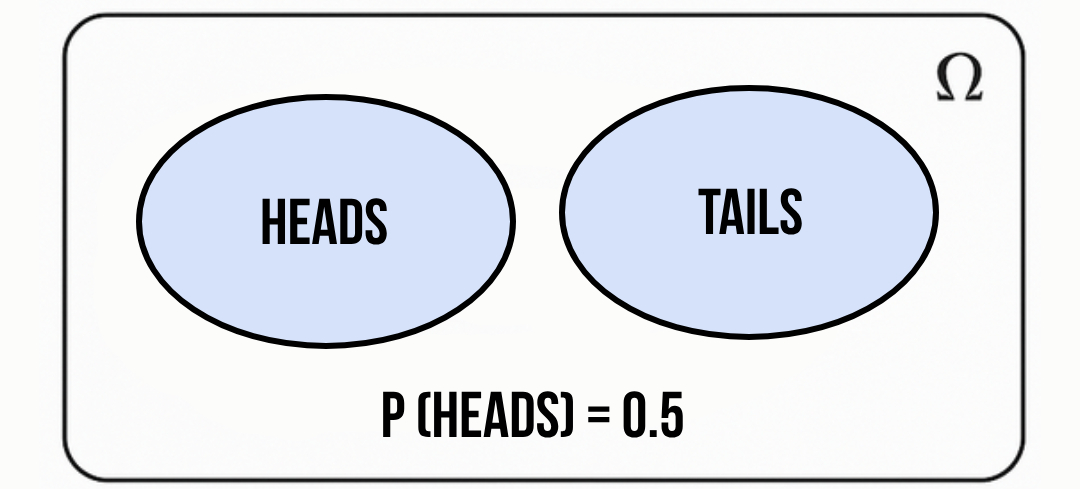
\includegraphics[width=\linewidth]{chapter_figs/01_figs/space.jpg}
	\end{columns}
	\begin{itemize}
		\item $\Omega$ – All possible outcomes. \\
		      \textit{Example:} $\Omega = \{\text{Heads}, \text{Tails}\}$
		\item $\mathcal{A}$ – Set of events (measurable subsets of $\Omega$). \\
		      \textit{Example:} $\{\emptyset, \{\text{Heads}\}, \{\text{Tails}\}, \Omega\}$
		\item $P$ – A function that assigns probabilities to events in $\mathcal{A}$, satisfying:\\
		      \quad $P(\Omega) = 1$, \quad $P(E) \geq 0$, \quad countable additivity
	\end{itemize}
	
	\vspace{0.5em}
	\textbf{Probability is a mathematical framework to measure uncertainty.}
\end{frame}

\begin{frame}{Sigma-Algebra}
  \begin{figure}[htbp]
		\centering
		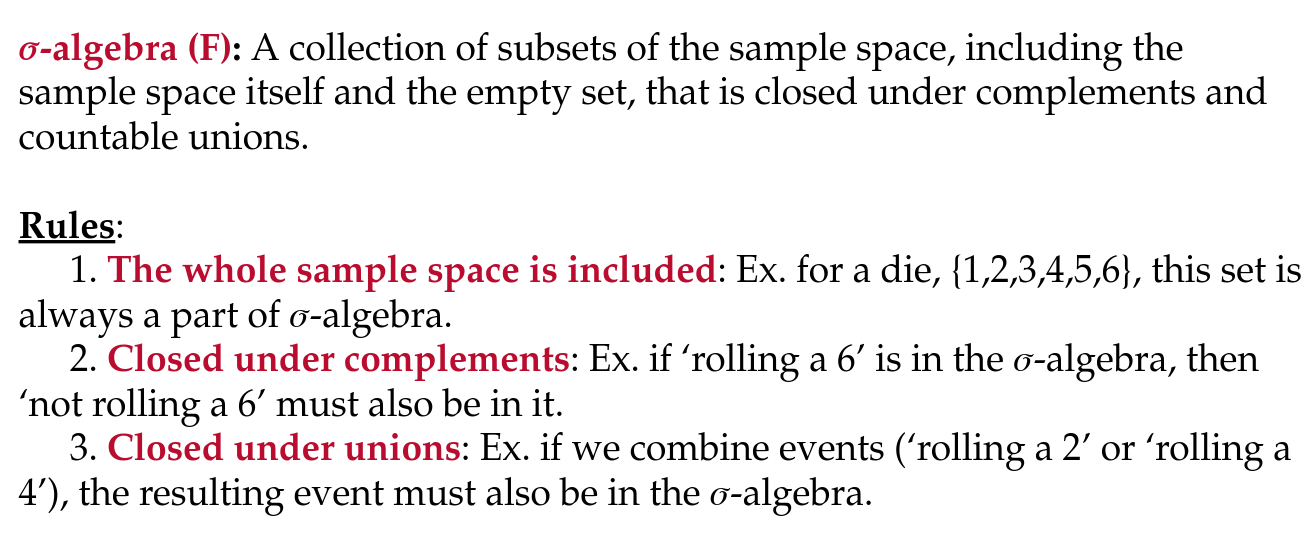
\includegraphics[width=\textwidth]{chapter_figs/01_figs/sigma_algebra.png}
	\end{figure}
\end{frame}

\begin{frame}{What is a Random Variable?}
	\textbf{A Random Variable (RV) assigns a number to each outcome in a sample space.}
	
	\vspace{1em}
	\begin{columns}
		\column{0.6\textwidth}
		\begin{itemize}
			\item Technically: A measurable function $X: \Omega \rightarrow \mathbb{R}$
			\item $X$ is the variable; $x$ is the value it takes (realization)
			\item \textit{Example:} Tossing a coin\\
			      \quad $\Omega = \{\text{Heads}, \text{Tails}\}$\\
			      \quad Define $X(\text{Heads}) = 1$, $X(\text{Tails}) = 0$
		\end{itemize}
		
		\vspace{0.5em}
		\textbf{RV turns uncertain outcomes into usable numbers.}
		
		\column{0.4\textwidth}
		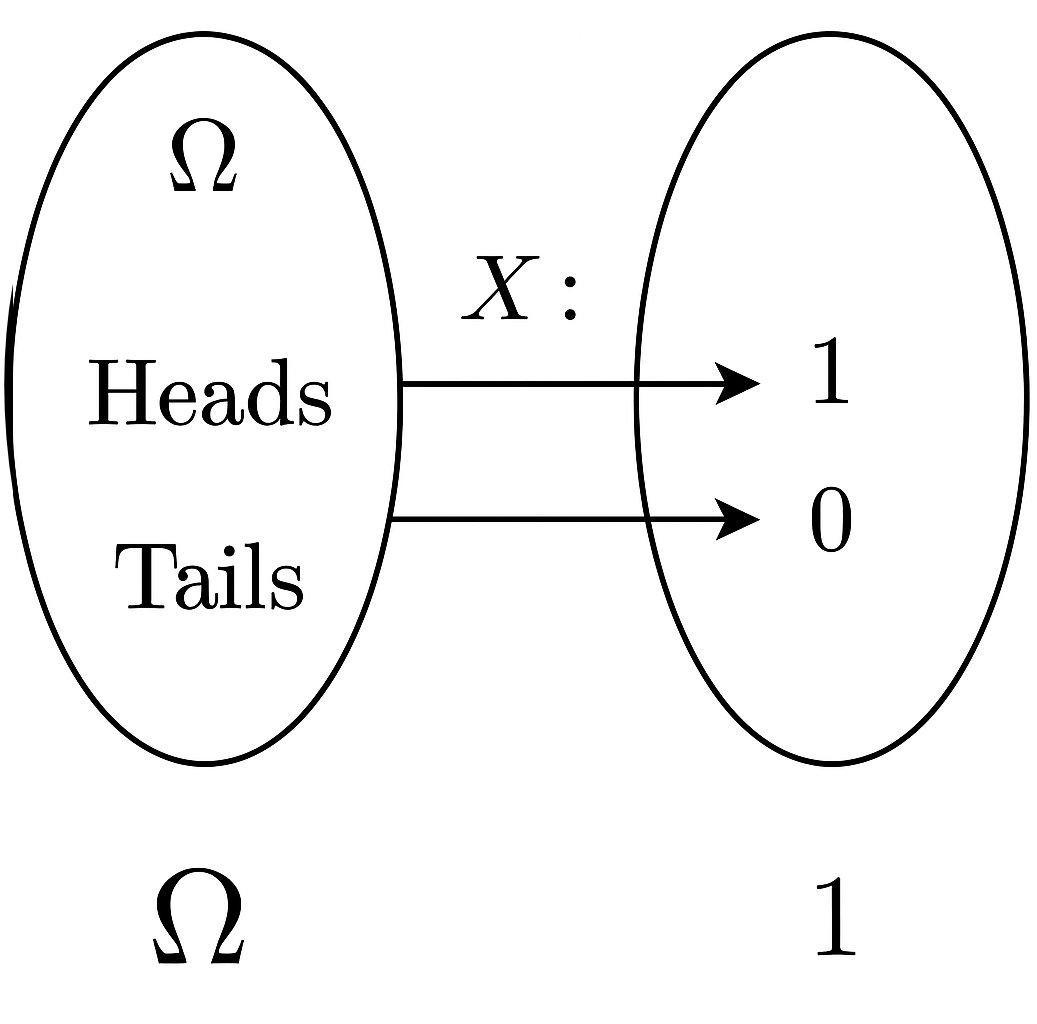
\includegraphics[width=\linewidth]{chapter_figs/01_figs/rv_mapping.png}
	\end{columns}
\end{frame}

\begin{frame}{What is a Probability Distribution?}
	\textbf{A probability distribution tells us how likely each outcome is.}
	\begin{columns}
		\column{0.6\textwidth}
		\begin{itemize}
			\item For discrete random variables -> we use a \textbf{PMF (Probability Mass Function)}. \textit{Example:} Rolling a die \\
			      \quad $P(X=3) = \frac{1}{6}$
			\item For continuous random variables -> use a \textbf{PDF (Probability Density Function)}. \textit{Example:} Gaussian distribution over real numbers\\
			      \quad $P(X = x) = 0$, but we can compute $P(a < X < b)$
			                      
		\end{itemize}
		              
		\column{0.4\textwidth}
		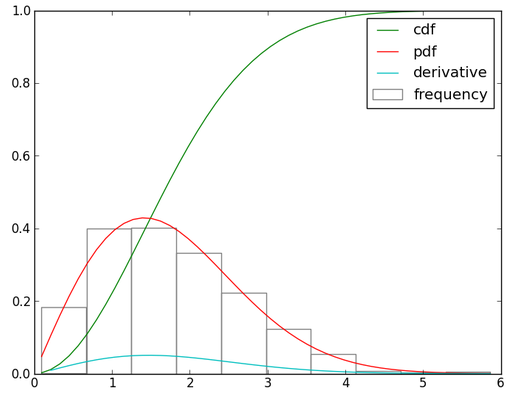
\includegraphics[width=\linewidth]{chapter_figs/01_figs/probability_distribution.png}
	\end{columns}
	    
	\begin{itemize}
		\item \textbf{CDF (Cumulative Distribution Function)} gives probability up to a value:\\
		      \quad $F(x) = P(X \leq x)$
	\end{itemize}
	\vspace{0.5em}
	\textbf{Distributions summarize how random variables behave.}
\end{frame}

\begin{frame}{What is a Continuous Distribution?}
	\textbf{In a continuous world, outcomes can't be counted — they fill an entire range.}
	
	\vspace{0.8em}
	\textbf{Discrete:} When we roll a die -> only 6 outcomes.\\
	\textbf{Continuous:} When we measure temperature -> infinite possibilities!
	
	\vspace{1em}
	\textbf{Key idea:} We talk about probability \textit{over intervals}, not single points.
	
	\vspace{1em}
	\[
		P(X = x) = 0 \quad \text{but} \quad P(a < X < b) > 0
	\]
	
	\vspace{0.8em}
	\textbf{Example:} Height of a person: $P(X = 170 \text{cm}) = 0$,\\
	but $P(169.5 < X < 170.5) > 0$
\end{frame}

\begin{frame}{Probability Density Function (PDF)}
	\textbf{A PDF describes how "dense" the probability is at each point.}
	
	\vspace{1em}
	\[
		P(a < X < b) = \int_a^b f(x) \, dx
	\]
	\textit{Where $f(x)$ is the PDF (e.g., bell curve)}
	
	\vspace{1em}
	\begin{columns}
		\column{0.6\textwidth}
		\begin{itemize}
			\item The PDF can be greater than 1! It’s not probability itself
			\item The \textbf{area under the curve} = probability
			\item Total area under the PDF = 1
		\end{itemize}
		  
		\column{0.4\textwidth}
		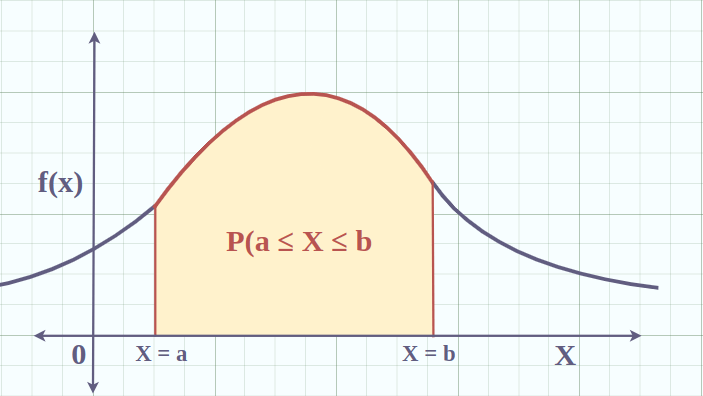
\includegraphics[width=\linewidth]{chapter_figs/01_figs/pdf.png}
	\end{columns}
	  
	
	\vspace{0.5em}
	\textbf{Think of it like mass spread over a continuous line.}
\end{frame}

\begin{frame}{Joint Probability}
	\textbf{Joint probability} describes the chance of two things happening together.
	
	\vspace{1em}
	\begin{columns}
		\column{0.6\textwidth}
		\textbf{Example:} Weather ($X$) and whether I carry an umbrella ($Y$)
		  
		\vspace{0.5em}
		\[
			P(X = \text{Rain},\; Y = \text{Yes}) = 0.3
		\]
		  
		\vspace{0.5em}
		\textbf{Notation:} $P(X, Y)$ or $P(X = x,\; Y = y)$
		
		\vspace{1em}
		\textbf{Joint distribution} is like a table of co-occurring probabilities.
		  
		\vspace{0.5em}
		  
		\column{0.4\textwidth}
		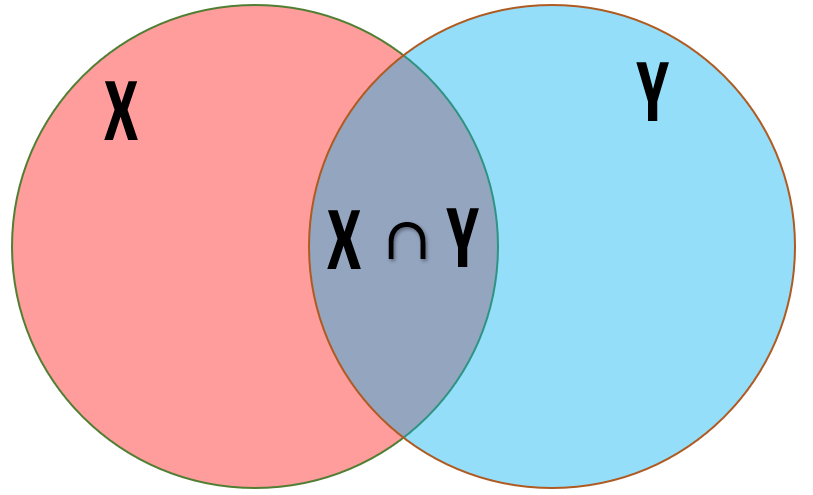
\includegraphics[width=\linewidth]{chapter_figs/01_figs/joint_probability_diagram.png}
	\end{columns}
	  
	\textit{We'll use this table on the next slide to compute marginal probabilities.}
\end{frame}

\begin{frame}{Marginalization (Sum Rule)}
	\textbf{Marginal probability} is the probability of one variable, \textit{ignoring} the other.
	
	\vspace{1em}
	\begin{align*}
		P(X = \text{Rain}) & = \sum_y P(X = \text{Rain}, Y = y)                               \\
		                   & = P(X=\text{Rain}, Y=\text{Yes}) + P(X=\text{Rain}, Y=\text{No}) 
	\end{align*}
	\vspace{0.5em}
	\textbf{Example:} Add across all umbrella choices.
	
	\vspace{0.5em}
	This process is called \textit{marginalization} — you're "summing out" a variable.
	
	\vspace{1em}
	\textbf{Visual:} We'll use a probability table and highlight the row/column.
\end{frame}

\begin{frame}{Conditional Probability}
  \textbf{Conditional probability is the probability of an event, given that another has happened.}

  \vspace{1em}
  \begin{columns}
    \column{0.6\textwidth}
\[
    P(A \mid B) = \frac{P(A \cap B)}{P(B)} \quad \text{(if } P(B) > 0\text{)}
  \]

  \vspace{1em}
  \textbf{Example:} What is the chance it’s raining \textit{given} we see someone with an umbrella?
  
    \column{0.4\textwidth}
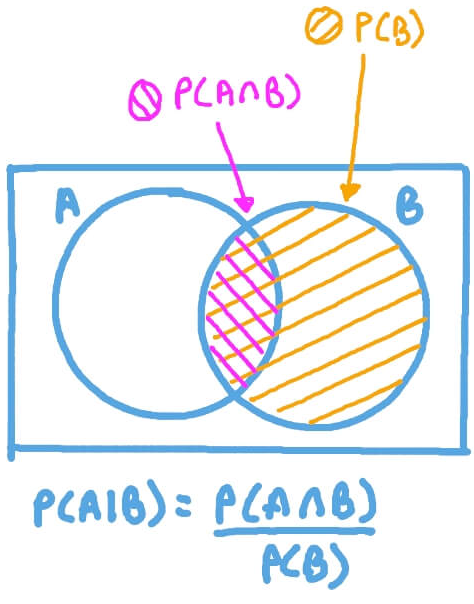
\includegraphics[width=0.6\linewidth]{chapter_figs/01_figs/conditional.png}
    
\end{columns}
  

  \vspace{1em}
  \textbf{Intuition (by my mathematics teacher):} We are zooming in on the part of the world where $B$ is true, and asking how often $A$ also happens.
\end{frame}

\begin{frame}{Bayes' Rule: Flipping the Condition}
  \textbf{The product rule:}
  \[
    P(A \cap B) = P(A \mid B) \cdot P(B)
  \]

  \vspace{1em}
  \textbf{Bayes' Rule:}
  \[
    P(A \mid B) = \frac{P(B \mid A) \cdot P(A)}{P(B)}
  \]

  \vspace{1em}
  \textbf{Why it matters:} Sometimes it's easier to compute $P(B \mid A)$ and $P(A)$ than $P(A \mid B)$ directly.

  \vspace{1em}
  \textbf{Used in:}
  \begin{itemize}
    \item Medical diagnosis
    \item Spam filters
    \item Weather prediction
  \end{itemize}
\end{frame}

\begin{frame}{Understanding Independence}
  \textbf{Two events are independent if knowing one tells us nothing about the other.}

  \vspace{1em}
  \[
    A \perp B \quad \Leftrightarrow \quad P(A \cap B) = P(A) \cdot P(B)
  \]

  \vspace{1em}
  \begin{columns}
    \column{0.6\textwidth}
\textbf{Example:} Tossing two fair coins:\\
  \quad $A$: First coin is heads \quad $P(A) = 0.5$\\
  \quad $B$: Second coin is heads \quad $P(B) = 0.5$\\
  \quad $P(A \cap B) = 0.25 = 0.5 \times 0.5$
  
    \column{0.4\textwidth}
    
\includegraphics[width=0.6\linewidth]{chapter_figs/01_figs/toss.png}
\end{columns}
  

  \vspace{1em}
  \textit{Knowing the result of one coin doesn’t affect the other. That’s independence!}
\end{frame}

\begin{frame}{Conditional Independence}
  \textbf{Conditional independence:} Two events are independent, given a third.

  \vspace{1em}
  \[
    A \perp B \mid C \quad \Leftrightarrow \quad P(A, B \mid C) = P(A \mid C) \cdot P(B \mid C)
  \]

  \vspace{1em}
  \begin{columns}
    \column{0.6\textwidth}
\textbf{Example:} Sprinkler (S) and Rain (R) both influence Wet Grass (W).\\
  The events S and R are independent. S doesn't depend on whether it is raining. Similarly, Raining doesn't depend on whether it is Sprinkling.

  \vspace{0.5em}
  $P(S,R) = P(S) \cdot P(R)$
  
    \column{0.4\textwidth}
    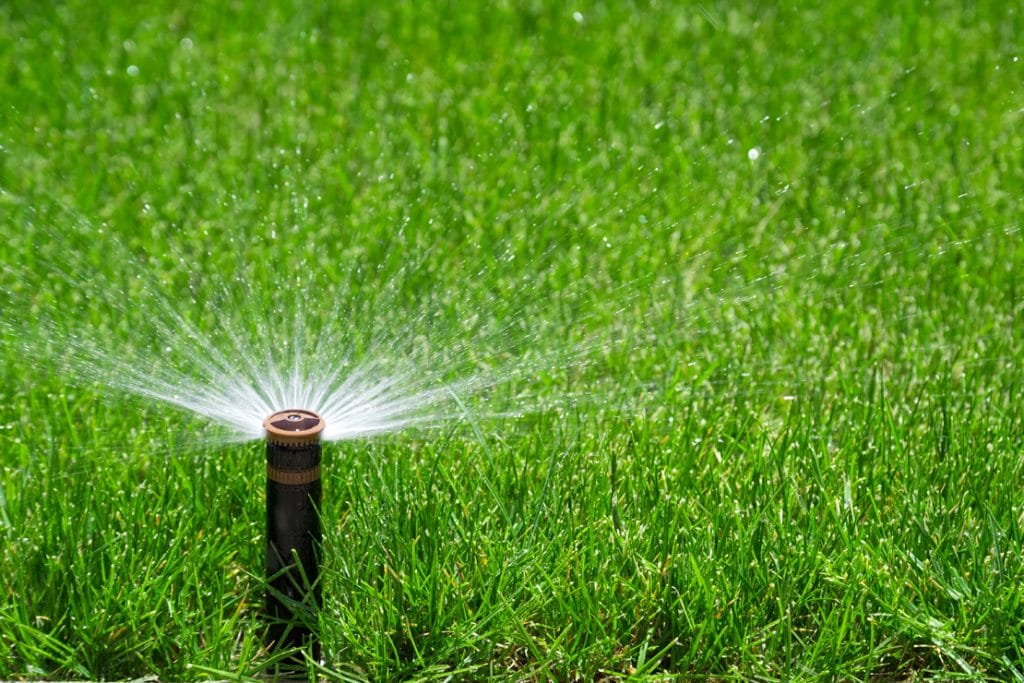
\includegraphics[width=\linewidth]{chapter_figs/01_figs/grass.jpg}
\end{columns}
  

  \vspace{1em}
  \textbf{Conditional independence is key in graphical models.}
\end{frame}

\begin{frame}{Directed Graphical Models}
  \textbf{Also called Bayesian Networks.}

  \vspace{1em}
  \textbf{Idea:} Use a directed graph to represent random variables and their dependencies.

  \vspace{1em}
  \begin{columns}
    \column{0.6\textwidth}

  \begin{itemize}
    \item Nodes = Random Variables
    \item Arrows = Direct influence / causal connection
  \end{itemize}

  \vspace{1em}
  \textbf{Why useful?}
  \begin{itemize}
    \item Makes complex distributions manageable
    \item Helps with reasoning and computation
  \end{itemize}
  
    \column{0.4\textwidth}
    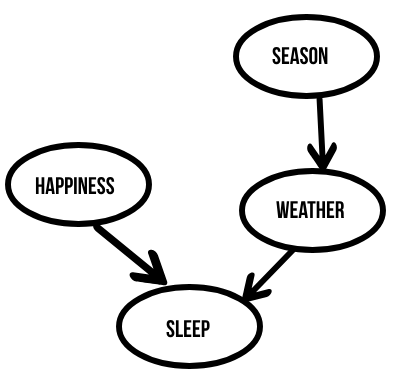
\includegraphics[width=\linewidth]{chapter_figs/01_figs/directed_graph.png}
\end{columns}

\end{frame}

\begin{frame}{Factorizing a Joint Distribution}
    \begin{figure}[htbp]
		\centering
		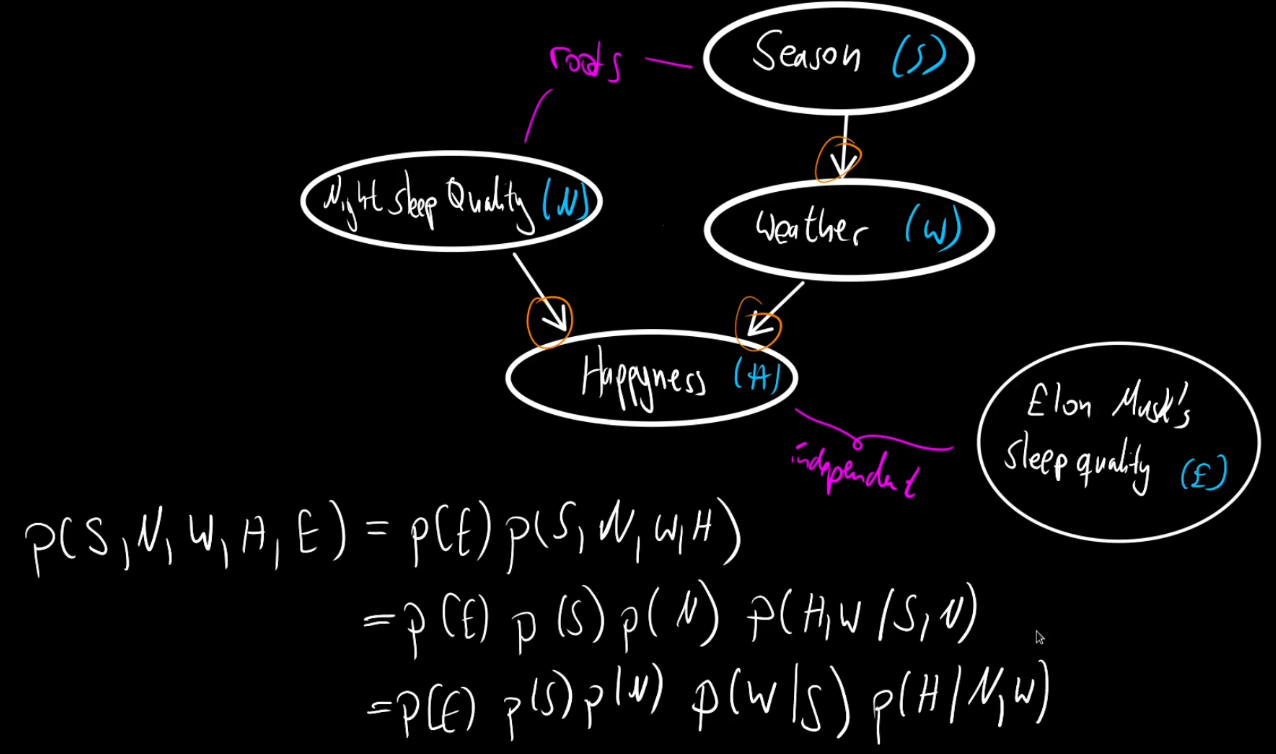
\includegraphics[width=0.8\textwidth]{chapter_figs/01_figs/factorization.png}
	\end{figure}
\end{frame}

\begin{frame}{Expectation (Expected Value)}
  \textbf{The expected value is the average outcome you'd expect in the long run.}
\vspace{1em}
    \begin{columns}
    \column{0.6\textwidth}
    
  \textbf{For discrete variables:}
  \[
    \mathbb{E}[X] = \sum_x x \cdot P(X = x)
  \]

  \textbf{For continuous variables:}
  \[
    \mathbb{E}[X] = \int_{-\infty}^{\infty} x \cdot f(x) \, dx
  \]
    \column{0.4\textwidth}
    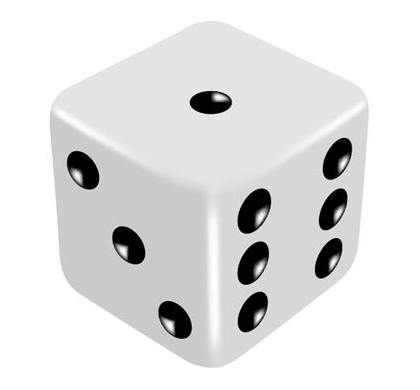
\includegraphics[width=0.5\linewidth]{chapter_figs/01_figs/dice.png}
\end{columns}

  

  \vspace{1em}
  \textbf{Example:} Roll a die $\rightarrow$ $\mathbb{E}[X] = 1\cdot \frac{1}{6} + 2\cdot \frac{1}{6} + 3\cdot \frac{1}{6} + \cdots + 6 \cdot \frac{1}{6} = 3.5$

  \vspace{1em}
  \textbf{Interpretation:} Think of it as the "center of gravity" of the distribution.
\end{frame}

\begin{frame}[plain]
	\begin{figure}[htbp]
		\centering
		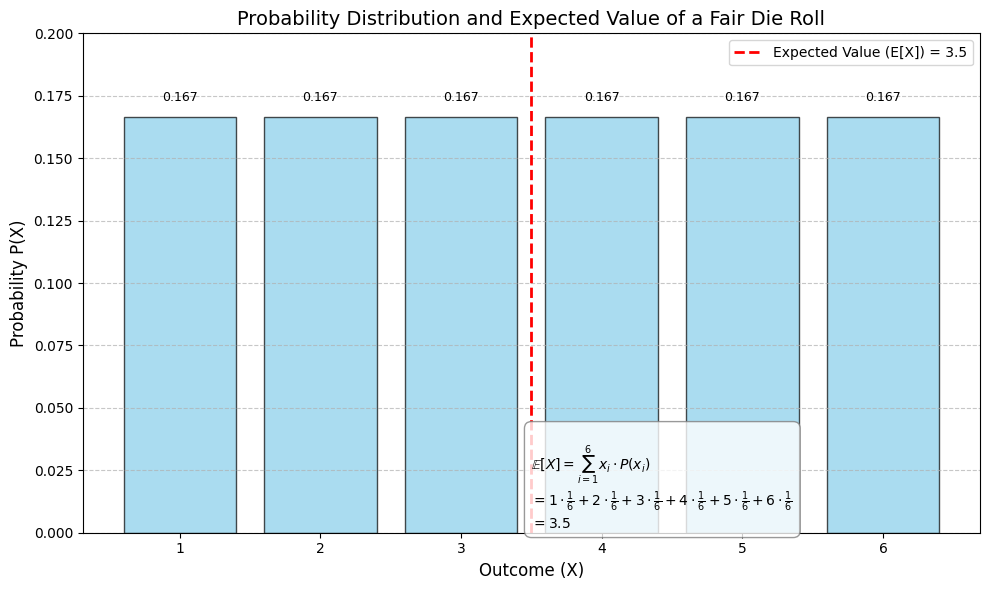
\includegraphics[width=\textwidth]{chapter_figs/01_figs/expectation.png}
	\end{figure}
\end{frame}

\begin{frame}{Variance – How Spread Out is the Distribution?}
  \textbf{Variance measures how much a random variable deviates from its mean.}

  \vspace{1em}
  \[
    \text{Var}(X) = \mathbb{E}[(X - \mathbb{E}[X])^2]
  \]
  \begin{columns}
    \column{0.6\textwidth}
\textbf{Standard deviation = } $\sqrt{\text{Var}(X)}$

  \vspace{1em}
  \textbf{Intuition:}
  \begin{itemize}
    \item High variance $\rightarrow$ outcomes are spread out
    \item Low variance $\rightarrow$ outcomes are close to the mean
  \end{itemize}
    \column{0.4\textwidth}
    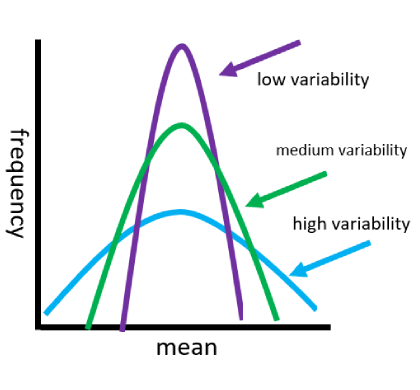
\includegraphics[width=0.7\textwidth]{chapter_figs/01_figs/variance.png}
\end{columns}

  

  \vspace{1em}
  \textit{Imagine measuring the heights of basketball players vs. chess players!}
\end{frame}


\begin{frame}{Covariance – Relationship Between Two Variables}
  \textbf{Covariance measures how two variables vary together.}

  \vspace{1em}
  \[
    \text{Cov}(X, Y) = \mathbb{E}[(X - \mathbb{E}[X])(Y - \mathbb{E}[Y])]
  \]

  \textbf{Interpretation:}
  \begin{itemize}
    \item $\text{Cov}(X, Y) > 0$ $\rightarrow$ increase together
    \item $\text{Cov}(X, Y) < 0$ $\rightarrow$ one increases, the other decreases
    \item $\text{Cov}(X, Y) = 0$ $\rightarrow$ uncorrelated (but not always independent!)
  \end{itemize}

  \vspace{1em}
  \textbf{Bonus:} Correlation is normalized covariance.
\end{frame}

\begin{frame}[plain]
	\begin{figure}[htbp]
		\centering
		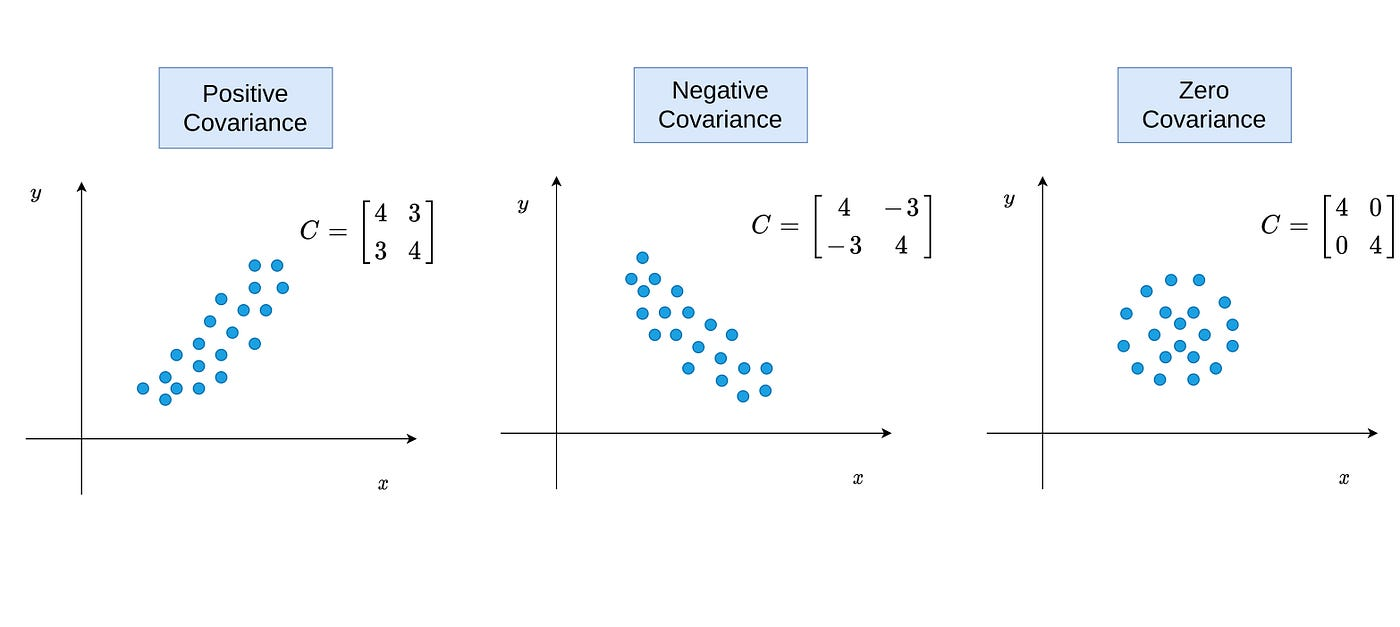
\includegraphics[width=\textwidth]{chapter_figs/01_figs/covariance.jpg}
	\end{figure}
\end{frame}

\begin{frame}{Change of Variables}
  \textbf{What if we transform a random variable into a new one?}
  \vspace{1em}
  \begin{figure}[htbp]
		\centering
		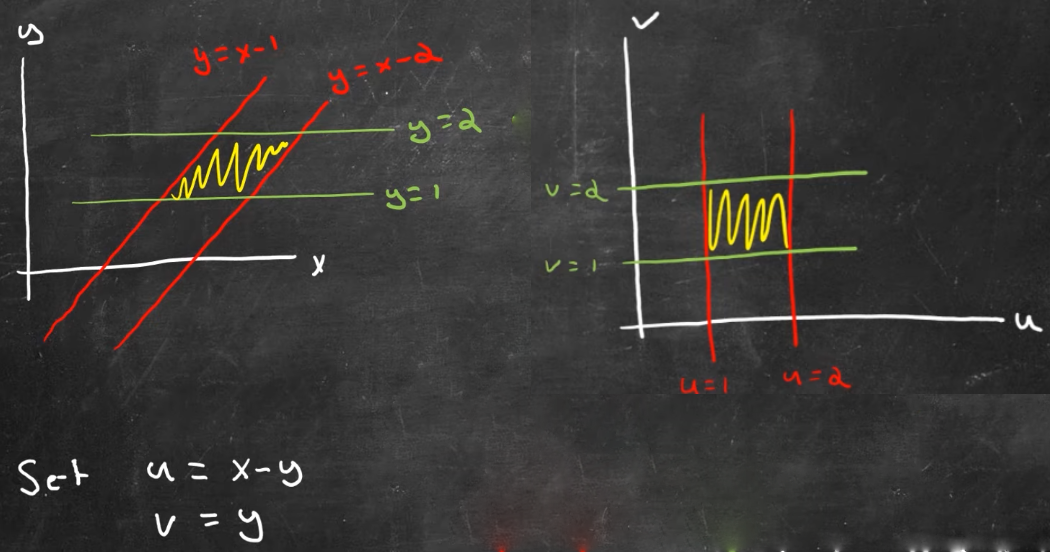
\includegraphics[width=0.8\textwidth]{chapter_figs/01_figs/change_of_variables.png}
	\end{figure}
  
\end{frame}

\begin{frame}{Change of Variables - 1D}
  \begin{figure}[htbp]
		\centering
		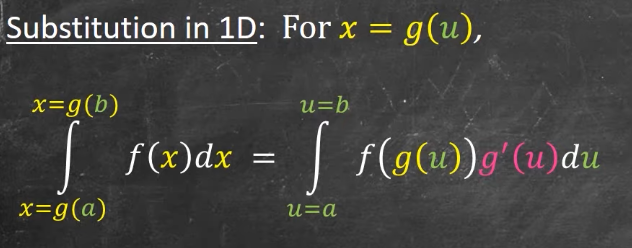
\includegraphics[width=0.8\textwidth]{chapter_figs/01_figs/1d.png}
	\end{figure}
  
\end{frame}

\begin{frame}{Change of Variables - 2D}
  \begin{figure}[htbp]
		\centering
		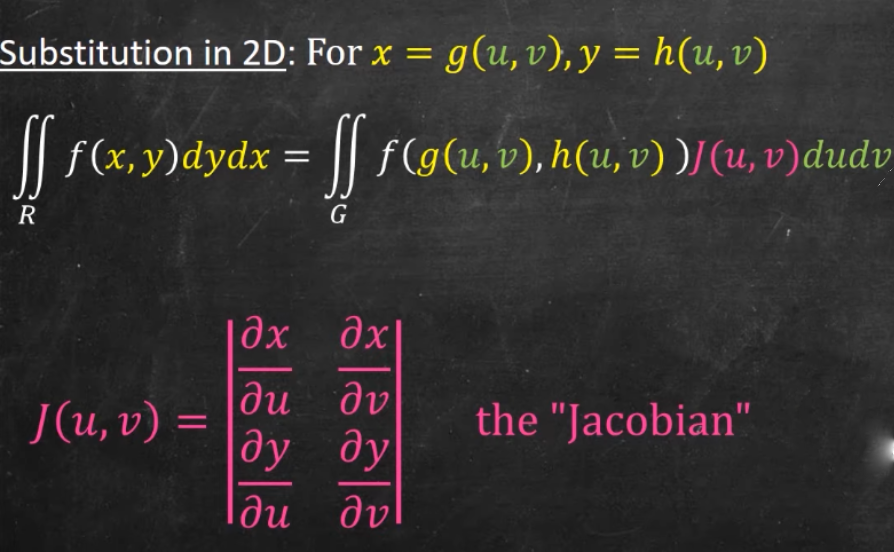
\includegraphics[width=0.8\textwidth]{chapter_figs/01_figs/2d.png}
	\end{figure}
  
\end{frame}

\begin{frame}{Plausible vs. Logical Inference}
  \textbf{Logical inference:} Uses strict rules — only what’s definitely true.\\
  \textbf{Plausible inference:} Operates under uncertainty — what's \textit{likely} true.

  \vspace{1em}
  \textbf{Example:}
  \begin{block}{Logical Inference}
    \textit{If it rains, the ground is wet.\\
    It is raining.\\
    $\Rightarrow$ The ground is wet.}
  \end{block}

  \begin{block}{Plausible Inference}
    \textit{The ground is wet.\\
    $\Rightarrow$ Maybe it rained? Maybe the sprinkler was on?}
  \end{block}

  \vspace{1em}
  \textbf{Key Insight:} Plausible inference lets us reason \textit{backwards} from evidence.\\
  This is the foundation of Bayesian thinking!
\end{frame}

\begin{frame}{Where Do Priors Come From?}
  \textbf{Priors} represent what we believe before seeing any data.

  \vspace{1em}
  \textbf{But where do they come from?}

    \begin{columns}
    \column{0.6\textwidth}
\begin{itemize}
    \item \textbf{Subjective belief:} Our personal knowledge or intuition.\\
    \textit{(e.g., “Coins are fair unless proven otherwise.”)}
    
    \item \textbf{Empirical estimates:} Based on past data.\\
    \textit{(e.g., “Spam words appear in 70\% of past spam emails.”)}
  \end{itemize}
  
    \column{0.4\textwidth}
    
\includegraphics[width=0.6\linewidth]{chapter_figs/01_figs/prior.png}
\end{columns}
  

  \vspace{1em}
  \textbf{Note:} Priors are not magic — they reflect assumptions. Make them wisely.
\end{frame}

\begin{frame}{What Are Conjugate Priors?}
  When you do Bayesian inference, you're updating a prior belief using data to get a posterior belief:

  \vspace{1em}
  \textbf{Bayes' Rule:}
  \[
    \text{Posterior} \propto \text{Likelihood} \times \text{Prior}
  \]

  \vspace{1em}
  Sometimes, after multiplying the prior and the likelihood, the result (posterior) belongs to the same family as the prior.

  \vspace{1em}
  That’s called a \textbf{conjugate prior}.
\end{frame}

\begin{frame}{Step 1 — Prior Belief}
  \textbf{We want to estimate the probability of heads, $\theta$, for a coin (baised).}

  \vspace{1em}
  \textbf{Before flipping the coin, we assume:}
  \[
    \theta \sim \text{Beta}(\alpha = 2,\; \beta = 2)
  \]

  \vspace{0.5em}
  This means:
  \begin{itemize}
    \item We believe the coin is fair (symmetric Beta)
    \item It’s like we've seen 1 head and 1 tail before
  \end{itemize}

  \vspace{1em}
  \textit{This is our prior belief. Now let’s collect data...}
\end{frame}

\begin{frame}{Step 2 — Observe Data}
  \textbf{We flip the coin 10 times and observe:}
  \[
    7 \text{ heads, } 3 \text{ tails}
  \]

  \vspace{1em}
  This is modeled as:
  \[
    X \sim \text{Binomial}(n = 10, \theta)
  \]

  \vspace{1em}
  \textit{Now we update our prior using Bayes' Rule...}
\end{frame}

\begin{frame}{Step 3 — Posterior Belief}
  \textbf{Using Bayes' Rule, our new belief is:}
  \[
    \theta \mid \text{data} \sim \text{Beta}(\alpha + \text{heads},\; \beta + \text{tails})
  \]

  \vspace{1em}
  In our case:
  \[
    \theta \mid \text{data} \sim \text{Beta}(2 + 7,\; 2 + 3) = \text{Beta}(9, 5)
  \]

  \vspace{1em}
  \textbf{Interpretation:}
  \begin{itemize}
    \item We've updated our belief based on observed data
    \item Posterior is still a Beta distribution — conjugacy!
  \end{itemize}

  \vspace{1em}
  \textit{This makes Bayesian updating fast and intuitive.}
\end{frame}

\begin{frame}{Tractable Gaussian Inference}
  \textbf{Gaussian distributions make Bayesian inference easy and exact.}

  \vspace{1em}
  \begin{columns}
    \column{0.6\textwidth}
Suppose we have:
  \[
    \theta \sim \mathcal{N}(\mu_0, \sigma_0^2) \quad \text{(Prior)}
  \]
  \[
    x \mid \theta \sim \mathcal{N}(\theta, \sigma^2) \quad \text{(Likelihood)}
  \]

  \vspace{1em}
  Then the posterior is also Gaussian:
  \[
    \theta \mid x \sim \mathcal{N}(\mu_{\text{post}}, \sigma_{\text{post}}^2)
  \]
  
    \column{0.4\textwidth}
    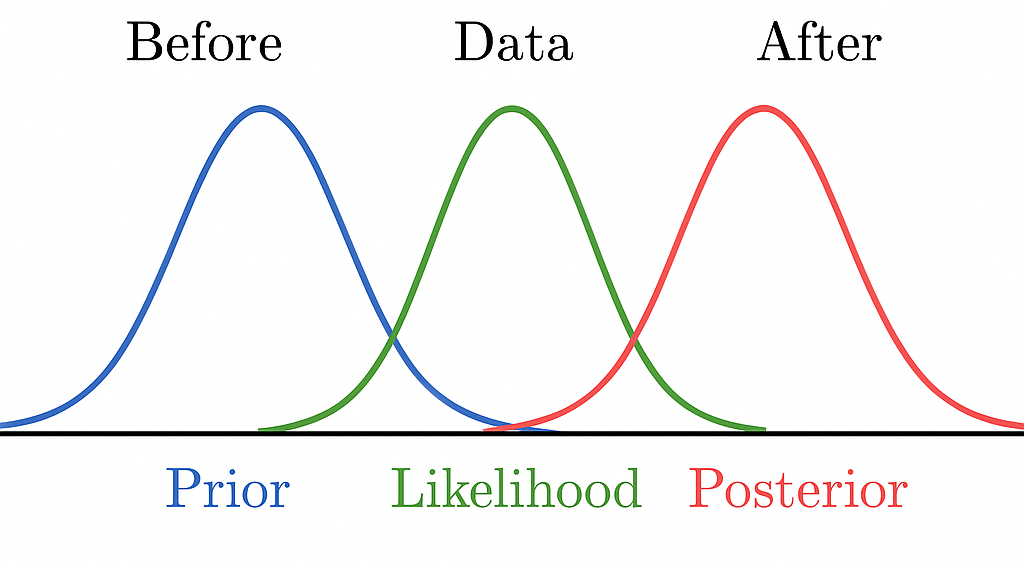
\includegraphics[width=0.8\linewidth]{chapter_figs/01_figs/gaussian.png}
\end{columns}
  

  \vspace{0.5em}
  \textbf{Key Benefits:}
  \begin{itemize}
    \item Conjugate: Gaussian prior + Gaussian likelihood = Gaussian posterior
    \item Easy to compute mean and variance updates
    \item Widely used in Kalman filters, linear regression, etc.
  \end{itemize}

\end{frame}


{\usebackgroundtemplate{
\includegraphics[width=\paperwidth]{chapter_figs/03_figs/thankyou.png}}
	\begin{frame}[plain,noframenumbering]
	\end{frame}}


\end{document}